\documentclass[conference]{IEEEtran}
\IEEEoverridecommandlockouts
% The preceding line is only needed to identify funding in the first footnote. If that is unneeded, please comment it out.
\usepackage{cite}
\usepackage{amsmath,amssymb,amsfonts}
\usepackage{algorithmic}
\usepackage{graphicx}
\usepackage{textcomp}
\usepackage{xcolor}
\def\BibTeX{{\rm B\kern-.05em{\sc i\kern-.025em b}\kern-.08em
    T\kern-.1667em\lower.7ex\hbox{E}\kern-.125emX}}
\begin{document}

\title{Parallel Matrix Multiplication\\
}

\author{\IEEEauthorblockN{Luca Falasca}
\IEEEauthorblockA{\textit{0334722} \\
luca.falasca@students.uniroma2.eu
}
\and
\IEEEauthorblockN{Matteo Conti}
\IEEEauthorblockA{\textit{0323728} \\
matteo.conti97@students.uniroma2.eu
}\\
}


\maketitle

\begin{abstract}
\end{abstract}

\section{Introduzione}
\subsection{Descrizione del problema}
Il progetto verte sulla realizzazione di un nucleo di calcolo per il prodotto tra due matrici, che sia quindi in grado di calcolare
$C \leftarrow C + AB$
dove A è una matrice $M$x$K$ e B è una matrice $K$x$N$. Per le matrici di input, si devono considerare due casi principali:
\begin{enumerate}
    \item Matrici quadrate $M = N = K$;
    \item Matrici rettangolari $M, N \gg K$; con $K = 32, 64, 128, 156$.
\end{enumerate}

\subsection{Obiettivi}

\subsection{Metriche di valutazione}
\subsection{Raccolta dei dati}
\section{MPI}
Nel constesto dell'HPC è fondamentale sfruttare le possibilità di parallelizzazione dei task da eseguire, in particolare in questa sezione verrà utilizzato il paradigma SIMD (Single Instruction Multiple Data) per la effettuare la moltiplicazione tra matrici utilizzando le funzionalità offerte da MPI per la parallelizzazione multiprocesso su CPU.\\ In particolare, verranno affrontati i seguenti problemi:
\begin{enumerate}
    \item Distribuzione del carico tra i processi
    \item Implementazione effettiva del prodotto tra matrici
\end{enumerate} 
\subsection{Distribuzione dei dati}
Per la distribuzione del carico è stata adottata una strategia simile a quella adottata dalla libreria ScaLAPACK, cioè la block cyclic distribution. Questa tecnica è caratterizzata principalmente da due aspetti:
\begin{itemize}
    \item I processi vengono visti come una griglia $P_r$x$P_c$
    \item La matrice viene divisa in blocchi di dimensione $B_r$x$B_c$
\end{itemize}
La griglia dei processi viene fatta scorrere lungo i blocchi con stride pari alla size della griglia, assegnando ad ogni processo $P_{i,j}$ un blocco $B_{i,j}$, ovviamente lo stesso processo in generale riceverà più di un blocco della matrice originale e non per forza tutti i processi riceveranno l'esatto numero di elementi, in particolare ogni processo riceve un blocco UxV con
%INSERIRE EQUAZIONE DOVE SI VEDE LA FORMULA PER U E V
Nel nostro caso le matrici sono state distribuite nel seguente modo:
\begin{itemize}
    \item La matrice A è stata distribuita in blocchi quadrati BxB (Fig. \ref{fig:matrix_a_distribution})
    \item La matrice B è stata distribuita in blocchi di righe BxK (Fig. \ref{fig:matrix_b_distribution}), in quanto ogni riga di dimensione B di un blocco della matrice A deve moltiplicare i primi B elementi di ogni colonna della matrice B, questo comporta che i processi nella stessa colonna della process grid debbano ricevere la stessa parte della matrice B
    \item La matrice C è stata distribuita in blocchi righe BxK (Fig. \ref{fig:matrix_c_distribution}), in quanto ogni processo deve calcolare un blocco di dimensione BxK della matrice C, questo comporta che i processi nella stessa riga della process grid debbano ricevere la stessa parte della matrice C
\end{itemize} 

\begin{figure}
    \centering
    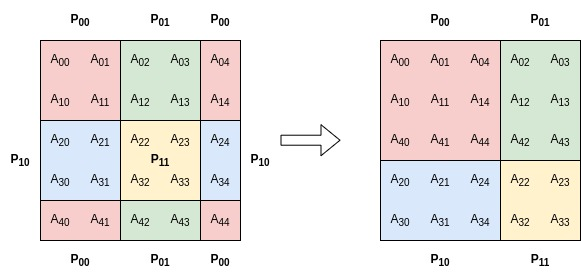
\includegraphics[width=0.5\textwidth]{resources/matrixA_2d_block_cyclic_distribution.jpg}
    \caption{Matrix A distribution.}
    \label{fig:matrix_a_distribution}
\end{figure}
\begin{figure}
    \centering
    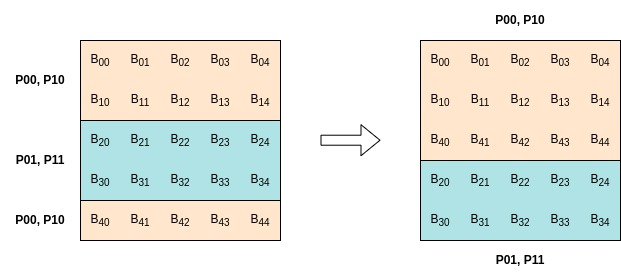
\includegraphics[width=0.5\textwidth]{resources/matrixB_row_block_cyclic_distribution.jpg}
    \caption{Matrix B distribution.}
    \label{fig:matrix_b_distribution}
\end{figure}
\begin{figure}
    \centering
    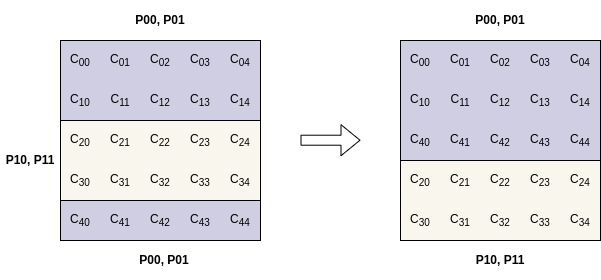
\includegraphics[width=0.5\textwidth]{resources/matrixC_row_block_cyclic_distribution.jpg}
    \caption{Matrix C distribution.}
    \label{fig:matrix_c_distribution}
\end{figure}
\subsection{Analisi delle prestazioni}

\section{CUDA}
Nel contesto dell'elaborazione parallela, l'impiego di unità di elaborazione grafica (GPU) ha rivoluzionato l'accelerazione di operazioni computazionali complesse, tra cui il calcolo matriciale. Questa sezione della relazione si concentra sull'implementazione del calcolo parallelo su GPU per la moltiplicazione di due matrici dense. La moltiplicazione di matrici dense è un'operazione fondamentale in numerose applicazioni scientifiche e di calcolo, tuttavia, il suo impatto computazionale può essere significativo, specialmente con matrici di grandi dimensioni. Pertanto, l'utilizzo delle architetture parallele delle GPU offre un'opportunità significativa per migliorare le prestazioni e ridurre i tempi di calcolo. In questa sezione verranno esaminate diverse implementazioni del prodotto tra matrici su GPU, con l'obiettivo di ottimizzare le prestazioni e ridurre i tempi di esecuzione.

\subsection{1 versione}
Nella presente iterazione del codice, si adotta un approccio procedurale mediante il quale la matrice A viene esaminata riga per riga, con ciascuna riga suddivisa per il numero di processi all'interno di un blocco. Analogamente, la matrice B subisce una suddivisione in base al numero di processi. Segue un ciclo in cui ogni processo elabora il proprio elemento della matrice A, effettuando la moltiplicazione con tutti i valori corrispondenti assegnati nella matrice B e sommandoli gradualmente per poi archiviarli in un vettore in memoria condivisa, con indice corrispondente all'identificativo del processo. Ciascun processo esegue tale operazione per tutti gli elementi della riga A che gli sono stati assegnati. Una volta completate le elaborazioni da parte di tutti i processi, si sincronizzano e sommano i risultati parziali ottenuti da ciascun processo mediante l'utilizzo di una funzione di riduzione. Tale procedura viene iterata per tutte le colonne della matrice B. Si è scelto di impiegare blocchi unidimensionali, dove ogni blocco è responsabile di una singola riga della matrice A. Pertanto, il numero di blocchi corrisponde al numero di righe della matrice A (m). (Fig. \ref{fig:cuda_scheme_v1})
\begin{figure}
    \centering
    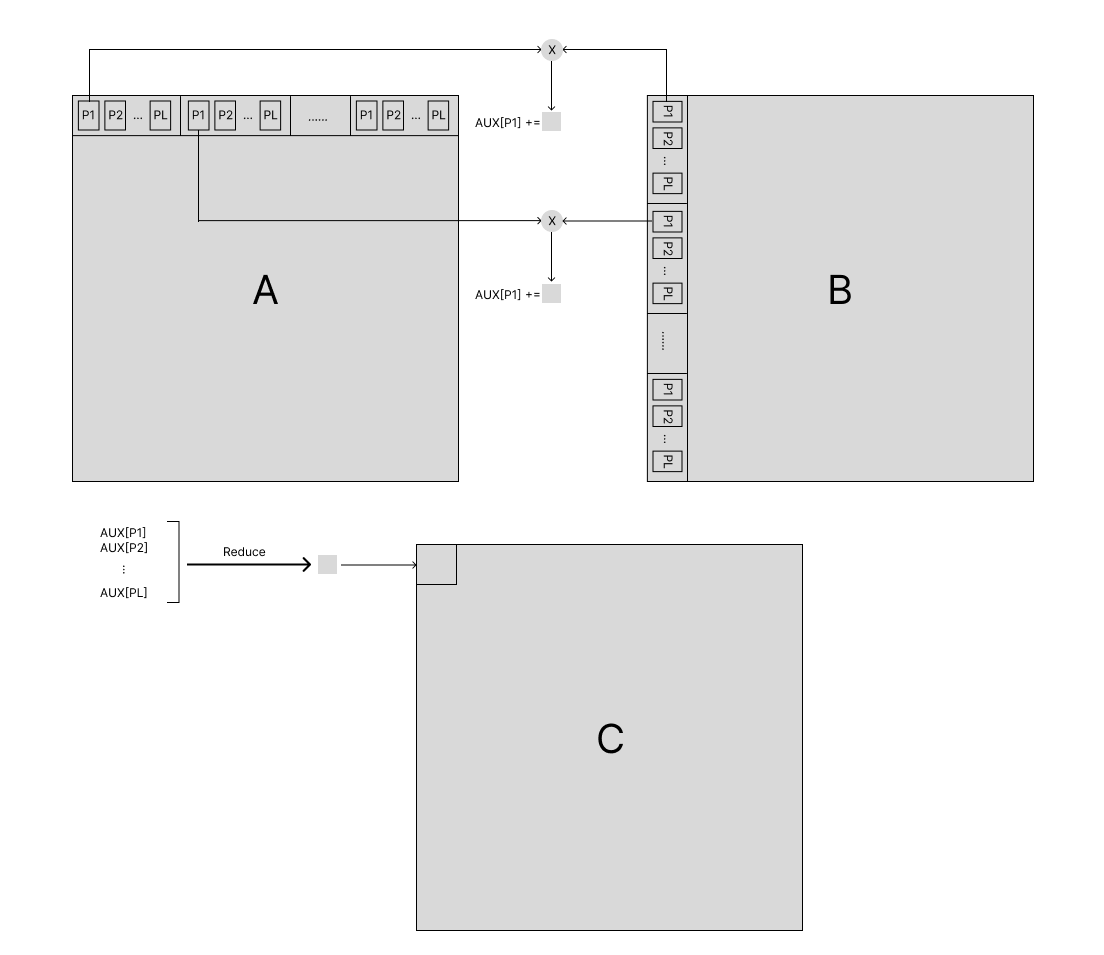
\includegraphics[width=0.5\textwidth]{resources/cuda_scheme_v1.png}
    \caption{Schema di funzionamento della prima versione del codice CUDA.}
    \label{fig:cuda_scheme_v1}
\end{figure}

\subsection{2 versione}
Poiché nella prima versione del codice si scriveva il risultato di un singolo elemento direttamente sulla matrice C ad ogni iterazione sulle colonne, e considerando che tra la fase di calcolo e quella di riduzione si richiedeva una sincronizzazione tra i thread, si è deciso di mitigare l'impatto di tali sincronizzazioni mediante l'adozione di un approccio che prevede l'elaborazione di gruppi di colonne per volta. Di conseguenza, i risultati parziali sono scritti su una matrice temporanea in memoria condivisa. Questa strategia consente di ridurre il numero di sincronizzazioni tra i thread richieste dall'algoritmo. (Fig. \ref{fig:cuda_scheme_v2})


\begin{figure}
    \centering
    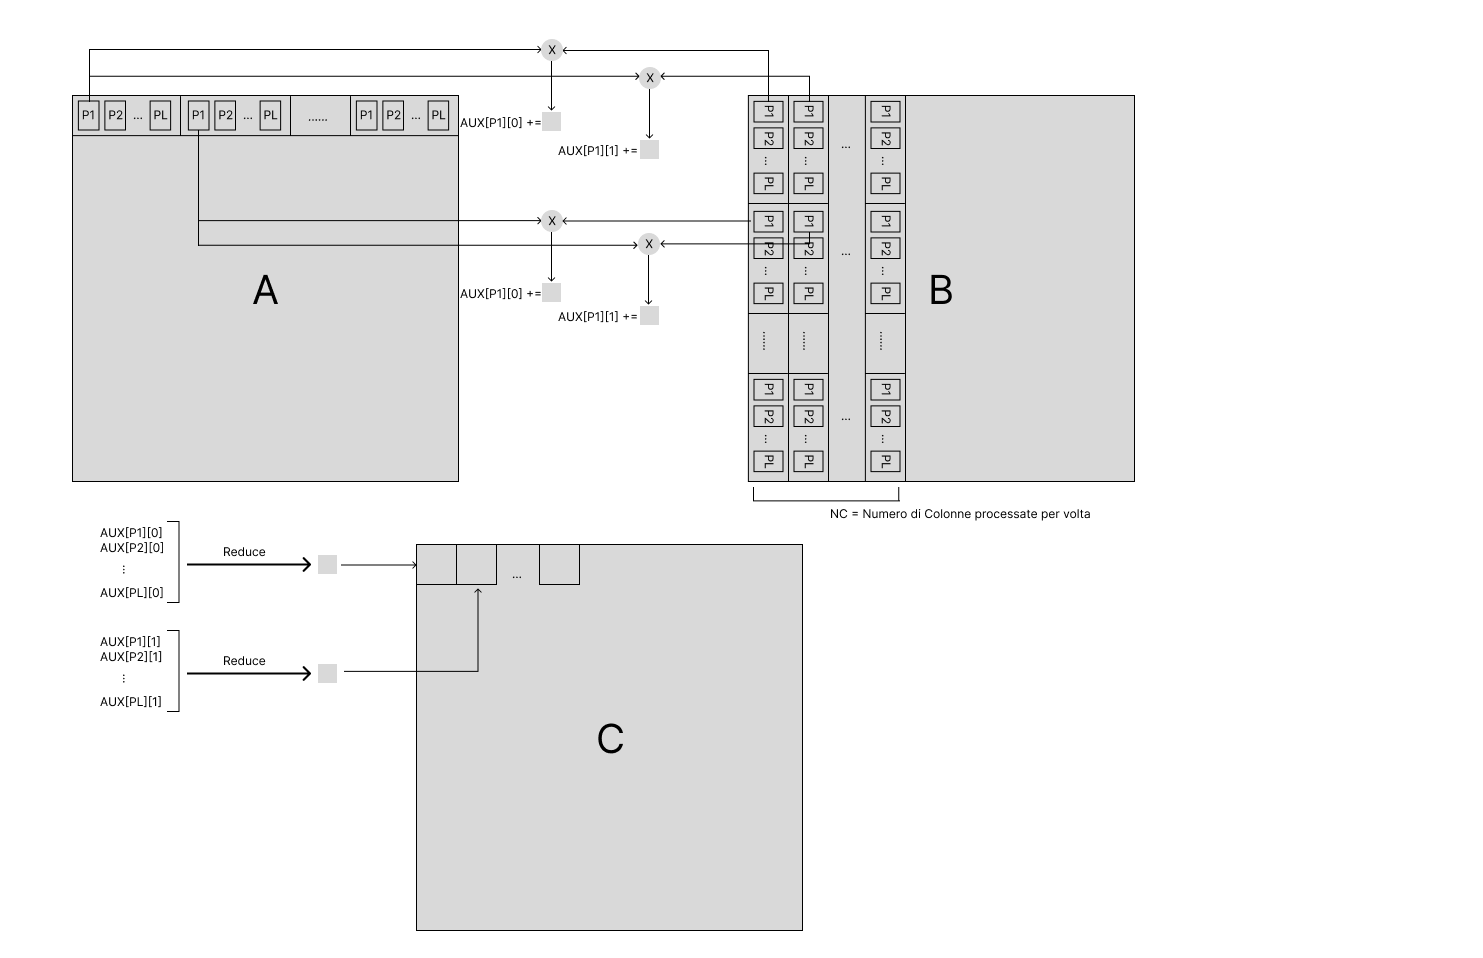
\includegraphics[width=0.5\textwidth]{resources/cuda_scheme_v2.png}
    \caption{Schema di funzionamento della seconda versione del codice CUDA.}
    \label{fig:cuda_scheme_v2}
\end{figure}

\subsection{3 versione}
Nella terza iterazione, si mira a sfruttare l'idea che durante ciascuna iterazione del prodotto tra una riga considerata e un gruppo di colonne, gli stessi elementi della riga A sono utilizzati ripetutamente. Questo consente di memorizzarli in memoria condivisa, riducendo così il numero complessivo di accessi alla memoria globale e incrementando l'efficienza dell'esecuzione. Tuttavia, l'implementazione iniziale prevede lo scorrimento di una colonna alla volta, il che implica la necessità di memorizzare l'intera riga in memoria condivisa. Questo approccio risulta poco pratico dato che le dimensioni delle righe sono considerevoli e la capacità della memoria condivisa è limitata. \\ Per risolvere questo problema, anziché iterare una colonna per volta, si è optato per l'iterazione sulla riga parziale del sottoinsieme delle colonne di B per volta. In questo modo, viene sfruttata la medesima porzione della riga A per eseguire il prodotto con le colonne di B. Tale strategia ottimizza l'utilizzo della memoria condivisa, garantendo al contempo un migliore bilanciamento tra l'efficienza computazionale e l'utilizzo delle risorse di memoria disponibili. (Fig. \ref{fig:cuda_scheme_v3})

\begin{figure}
    \centering
    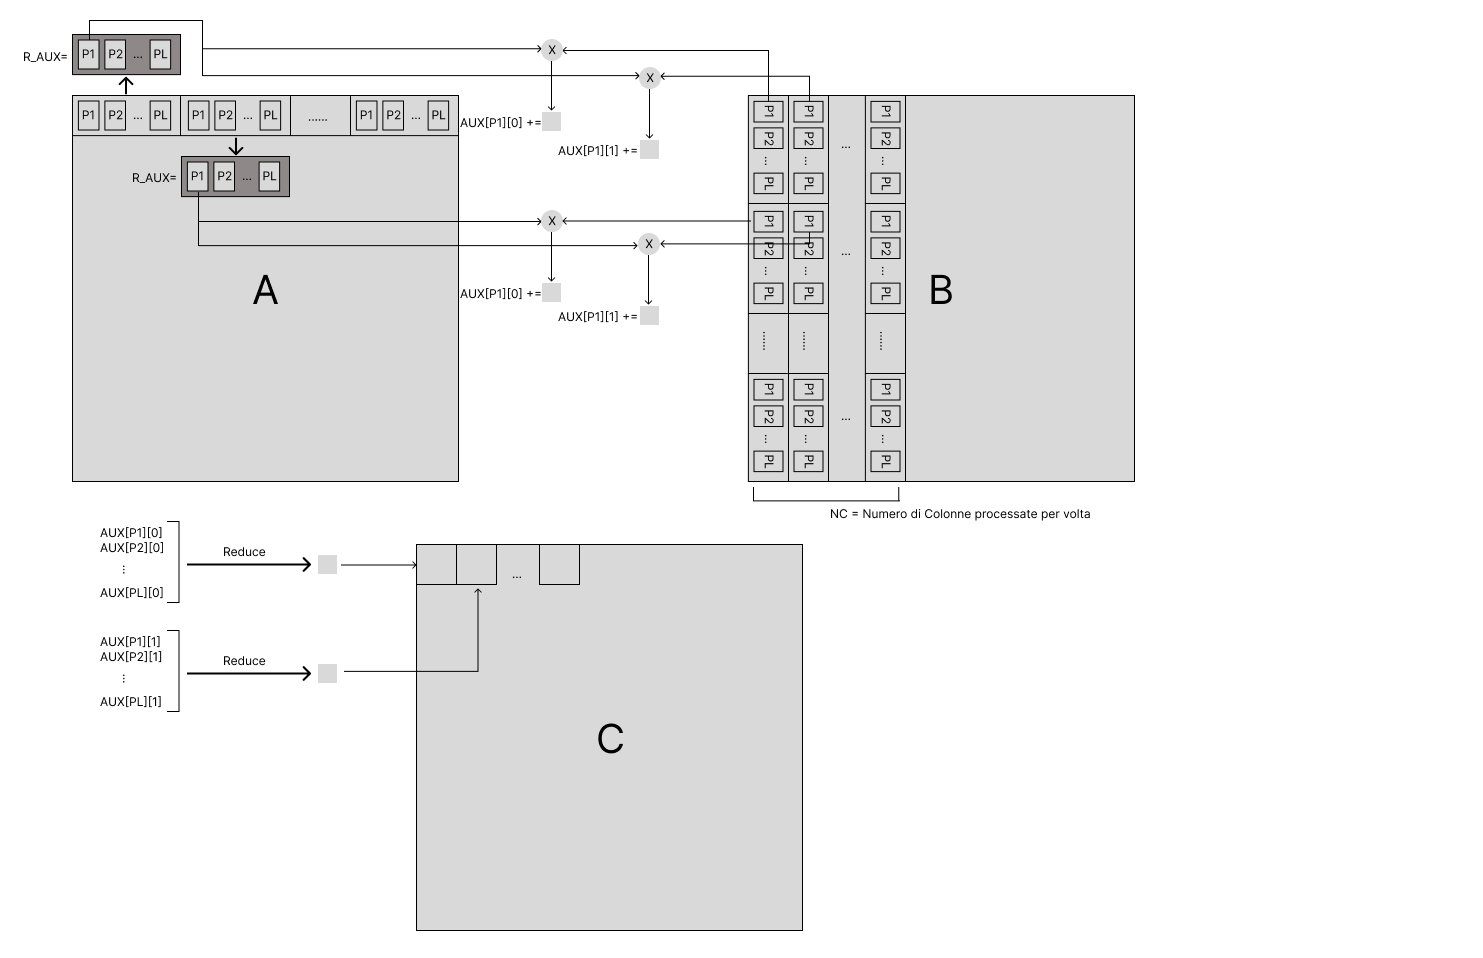
\includegraphics[width=0.5\textwidth]{resources/cuda_scheme_v3.png}
    \caption{Schema di funzionamento della terza versione del codice CUDA.}
    \label{fig:cuda_scheme_v3}ù
\end{figure}

\subsection{4 versione}
Nella quarta iterazione, si è introdotta una piccola variazione nel calcolo dell'indice di colonna di B, rispetto alla terza versione. Nella versione precedente, l'indice di colonna di B viene calcolato come $icx = i * k + j * k + ic$, dove $i$ indica la colonna in cui inizia il blocco di colonne corrente e $j$ rappresenta l'indice della colonna corrente all'interno del blocco. In questo modo, $ik$ posiziona l'iteratore all'inizio del blocco corrente, mentre $jk$ permette di navigare all'interno del blocco. \\ Nella nuova versione, si è scelto di raccogliere il termine $k$, riducendo così il numero di moltiplicazioni. L'indice di colonna di B viene calcolato come $icx = (i + j) * k + ic$. Questa variazione è stata mantenuta perché, nonostante sia una differenza minima, ha dimostrato di influenzare le performance in modo particolare, generando risultati distinti.
\subsection{Analisi delle prestazioni}
\section{Suddivisione del lavoro}
\section*{References}

Please number citations consecutively within brackets \cite{b1}. The 
sentence punctuation follows the bracket \cite{b2}. Refer simply to the reference 
number, as in \cite{b3}---do not use ``Ref. \cite{b3}'' or ``reference \cite{b3}'' except at 
the beginning of a sentence: ``Reference \cite{b3} was the first $\ldots$''

Number footnotes separately in superscripts. Place the actual footnote at 
the bottom of the column in which it was cited. Do not put footnotes in the 
abstract or reference list. Use letters for table footnotes.

Unless there are six authors or more give all authors' names; do not use 
``et al.''. Papers that have not been published, even if they have been 
submitted for publication, should be cited as ``unpublished'' \cite{b4}. Papers 
that have been accepted for publication should be cited as ``in press'' \cite{b5}. 
Capitalize only the first word in a paper title, except for proper nouns and 
element symbols.

For papers published in translation journals, please give the English 
citation first, followed by the original foreign-language citation \cite{b6}.

\begin{thebibliography}{00}
\bibitem{b1} G. Eason, B. Noble, and I. N. Sneddon, ``On certain integrals of Lipschitz-Hankel type involving products of Bessel functions,'' Phil. Trans. Roy. Soc. London, vol. A247, pp. 529--551, April 1955.
\bibitem{b2} J. Clerk Maxwell, A Treatise on Electricity and Magnetism, 3rd ed., vol. 2. Oxford: Clarendon, 1892, pp.68--73.
\bibitem{b3} I. S. Jacobs and C. P. Bean, ``Fine particles, thin films and exchange anisotropy,'' in Magnetism, vol. III, G. T. Rado and H. Suhl, Eds. New York: Academic, 1963, pp. 271--350.
\bibitem{b4} K. Elissa, ``Title of paper if known,'' unpublished.
\bibitem{b5} R. Nicole, ``Title of paper with only first word capitalized,'' J. Name Stand. Abbrev., in press.
\bibitem{b6} Y. Yorozu, M. Hirano, K. Oka, and Y. Tagawa, ``Electron spectroscopy studies on magneto-optical media and plastic substrate interface,'' IEEE Transl. J. Magn. Japan, vol. 2, pp. 740--741, August 1987 [Digests 9th Annual Conf. Magnetics Japan, p. 301, 1982].
\bibitem{b7} M. Young, The Technical Writer's Handbook. Mill Valley, CA: University Science, 1989.
\end{thebibliography}
\vspace{12pt}


\end{document}